\documentclass[tikz,border=2pt]{standalone}
\usepackage{amsmath,amssymb}
\usetikzlibrary{arrows.meta,positioning,calc,fit,backgrounds}
\begin{document}
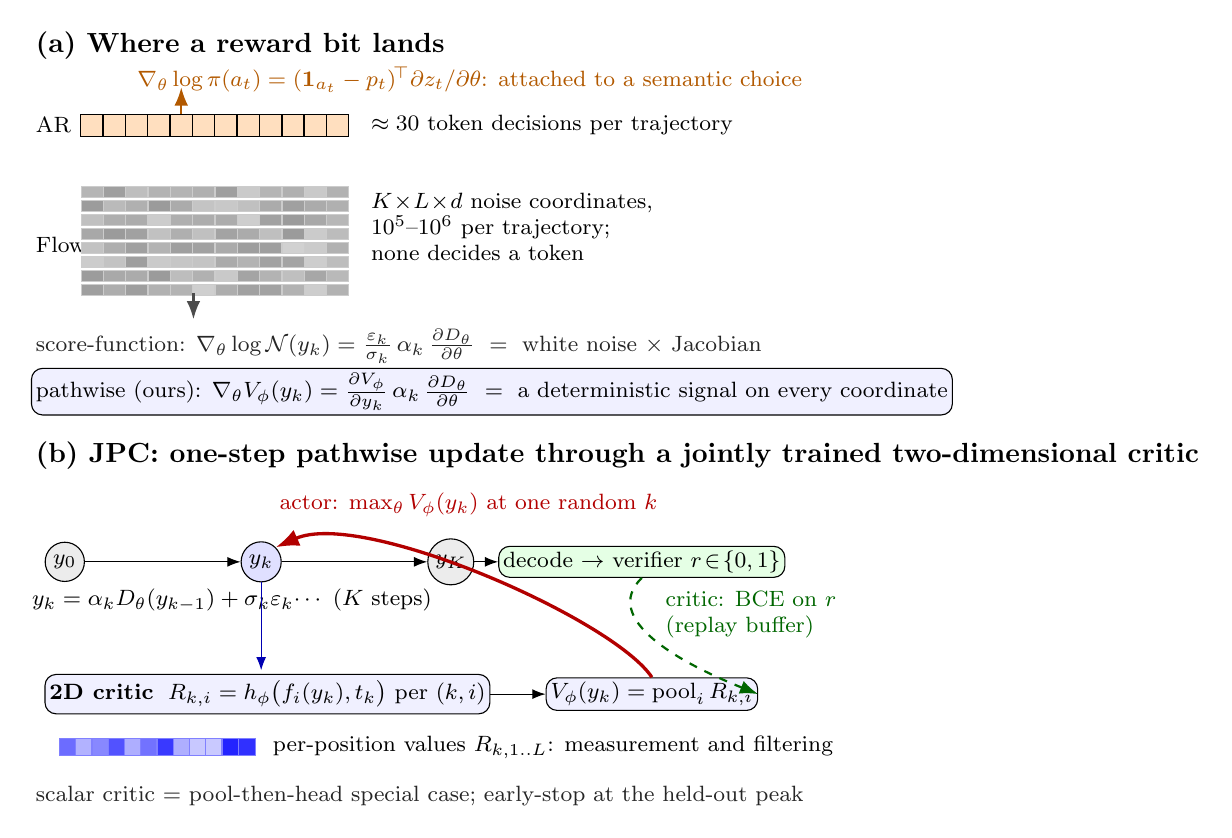
\begin{tikzpicture}[font=\footnotesize,>=Latex, every node/.style={inner sep=1.6pt}, x=0.86cm, y=1.12cm]
% ================= (a) =================
\node[font=\normalsize\bfseries,anchor=west] at (0,4.3) {(a) Where a reward bit lands};
\node[anchor=west] at (0,3.4) {AR};
\foreach \i in {0,...,11}{\node[draw,fill=orange!25,minimum width=0.28cm,minimum height=0.28cm,inner sep=0] (a\i) at (0.9+0.33*\i,3.4) {};}
\node[anchor=west] at (4.95,3.4) {$\approx 30$ token decisions per trajectory};
\draw[->,thick,orange!70!black] (a4.north) -- ++(0,0.3);
\node[anchor=south west,orange!70!black] at (1.5,3.72) {$\nabla_\theta \log\pi(a_t)=(\mathbf 1_{a_t}-p_t)^{\!\top}\partial z_t/\partial\theta$: attached to a semantic choice};
\node[anchor=west] at (0,2.05) {Flow};
\foreach \k in {0,...,7}{\foreach \j in {0,...,11}{\pgfmathsetmacro{\g}{35+45*rnd}
  \node[draw=gray!40,fill=gray!\g,minimum width=0.28cm,minimum height=0.14cm,inner sep=0,line width=0.2pt] at (0.9+0.33*\j,2.65-0.16*\k) {};}}
\node[anchor=west,align=left] at (4.95,2.25) {$K\!\times\!L\!\times\!d$ noise coordinates,\\ $10^{5}$--$10^{6}$ per trajectory;\\ none decides a token};
\draw[->,thick,gray!60!black] (2.4,1.5) -- ++(0,-0.3);
\node[anchor=north west,gray!30!black] at (0.0,1.15) {score-function: $\nabla_\theta\log\mathcal N(y_k)=\tfrac{\varepsilon_k}{\sigma_k}\,\alpha_k\,\tfrac{\partial D_\theta}{\partial\theta}$ \;=\; white noise $\times$ Jacobian};
\node[draw,rounded corners,fill=blue!6,anchor=north west,align=left] at (0.0,0.65) {pathwise (ours): $\nabla_\theta V_\phi(y_k)=\tfrac{\partial V_\phi}{\partial y_k}\,\alpha_k\,\tfrac{\partial D_\theta}{\partial\theta}$ \;=\; a deterministic signal on every coordinate};
% ================= (b) =================
\node[font=\normalsize\bfseries,anchor=west] at (0,-0.35) {(b) JPC: one-step pathwise update through a jointly trained two-dimensional critic};
\node[draw,circle,fill=gray!15,minimum size=0.42cm] (y0) at (0.5,-1.55) {$y_0$};
\node[draw,circle,fill=blue!12,minimum size=0.42cm] (yk) at (3.4,-1.55) {$y_k$};
\node[draw,circle,fill=gray!15,minimum size=0.42cm] (yK) at (6.2,-1.55) {$y_K$};
\node[draw,rounded corners,fill=green!10,anchor=west] (txt) at (6.9,-1.55) {decode $\to$ verifier $r\!\in\!\{0,1\}$};
\draw[->] (y0) -- (yk); \node[anchor=north] at (1.95,-1.8) {$y_{k}=\alpha_k D_\theta(y_{k-1})+\sigma_k\varepsilon_k$};
\draw[->] (yk) -- (yK); \node[anchor=north] at (4.9,-1.8) {$\cdots$ ($K$ steps)};
\draw[->] (yK) -- (txt);
\node[draw,rounded corners,fill=blue!6,minimum height=0.5cm,align=center,anchor=west] (cr) at (0.2,-3.05) {\textbf{2D critic}\; $R_{k,i}=h_\phi\big(f_i(y_k),t_k\big)$ per $(k,i)$};
\node[draw,rounded corners,fill=blue!6,anchor=west] (V) at (7.6,-3.05) {$V_\phi(y_k)=\mathrm{pool}_i\,R_{k,i}$};
\draw[->] (cr) -- (V);
\draw[->,blue!70!black] (yk.south) -- (3.4,-2.78);
\foreach \i in {0,...,11}{\pgfmathsetmacro{\g}{15+75*rnd}\node[draw=blue!50,fill=blue!\g!white,minimum width=0.22cm,minimum height=0.22cm,inner sep=0] at (0.55+0.24*\i,-3.65) {};}
\node[anchor=west] at (3.5,-3.65) {per-position values $R_{k,1..L}$: measurement and filtering};
\draw[->,red!70!black,very thick] (V.north) .. controls (8.6,-2.2) and (4.9,-0.95) .. (yk.north east);
\node[red!70!black,anchor=west] at (3.6,-0.9) {actor: $\max_\theta V_\phi(y_k)$ at one random $k$};
\draw[->,dashed,green!40!black,thick] (txt.south) .. controls (8.4,-2.2) and (9.6,-2.7) .. (V.east);
\node[green!40!black,anchor=west,align=left] at (9.3,-2.15) {critic: BCE on $r$\\ (replay buffer)};
\node[anchor=west,gray!30!black] at (0,-4.2) {scalar critic $=$ pool-then-head special case; early-stop at the held-out peak};
\end{tikzpicture}
\end{document}
